\documentclass[a0paper,portrait,25pt,margin=0.5in,innermargin=-4.5in,blockverticalspace=-0.25in]{tikzposter}

% essential physics, math and typing package
\usepackage[greek,english]{babel}
\usepackage{amsmath}
\usepackage{physics}

% other packages
\usepackage{enumitem}
\usepackage{lipsum} % dummy texts

% set theme 
\usepackage{nthu-theme}
\makeatletter
\setlength{\TP@visibletextwidth}{31.0in}
\setlength{\TP@visibletextheight}{45in}
\makeatother
% set theme parameters
\tikzposterlatexaffectionproofoff
\usetheme{NTHUTheme}
\usecolorstyle{NTHUStyle}

% set font parameters
\usepackage[T1]{fontenc}
\usepackage{unicode-math}
\setmainfont{TeX Gyre Heros}
\setmonofont{TeX Gyre Cursor}
\setmathfont{XITS Math}
\newfontfamily{\optima}{Optima}[
    Extension=.ttf,
    UprightFont=*-Regular,
    BoldFont=*-Bold,
]

% set header of poster
\title{\parbox{0.8\linewidth}{\optima NTHU Phys Poster Template - Example of a long title for a poster}}
\author{\LARGE \textbf{Yuan-Yen Peng}\textsuperscript{1,\dagger}, Siang-Yuan Lin\textsuperscript{1}, Pai-hsien Jennifer Hsu\textsuperscript{1},  Yun-Ju Lu\textsuperscript{1}}
\institute{\Large \textsuperscript{1}Department of Physics, National Tsing Hua University, Hsinchu, 30013, Taiwan.\\
\textsuperscript{\dagger}E-mail: \texttt{yuan-yen.peng@cern.ch}}
\titlegraphic{
\includegraphics[height=14cm]{PosterLogo.pdf}}

% begin document
\begin{document}
\maketitle
\centering

\begin{columns}

\column{0.5}

\block{Section 1}{
    
    \begin{align*}
        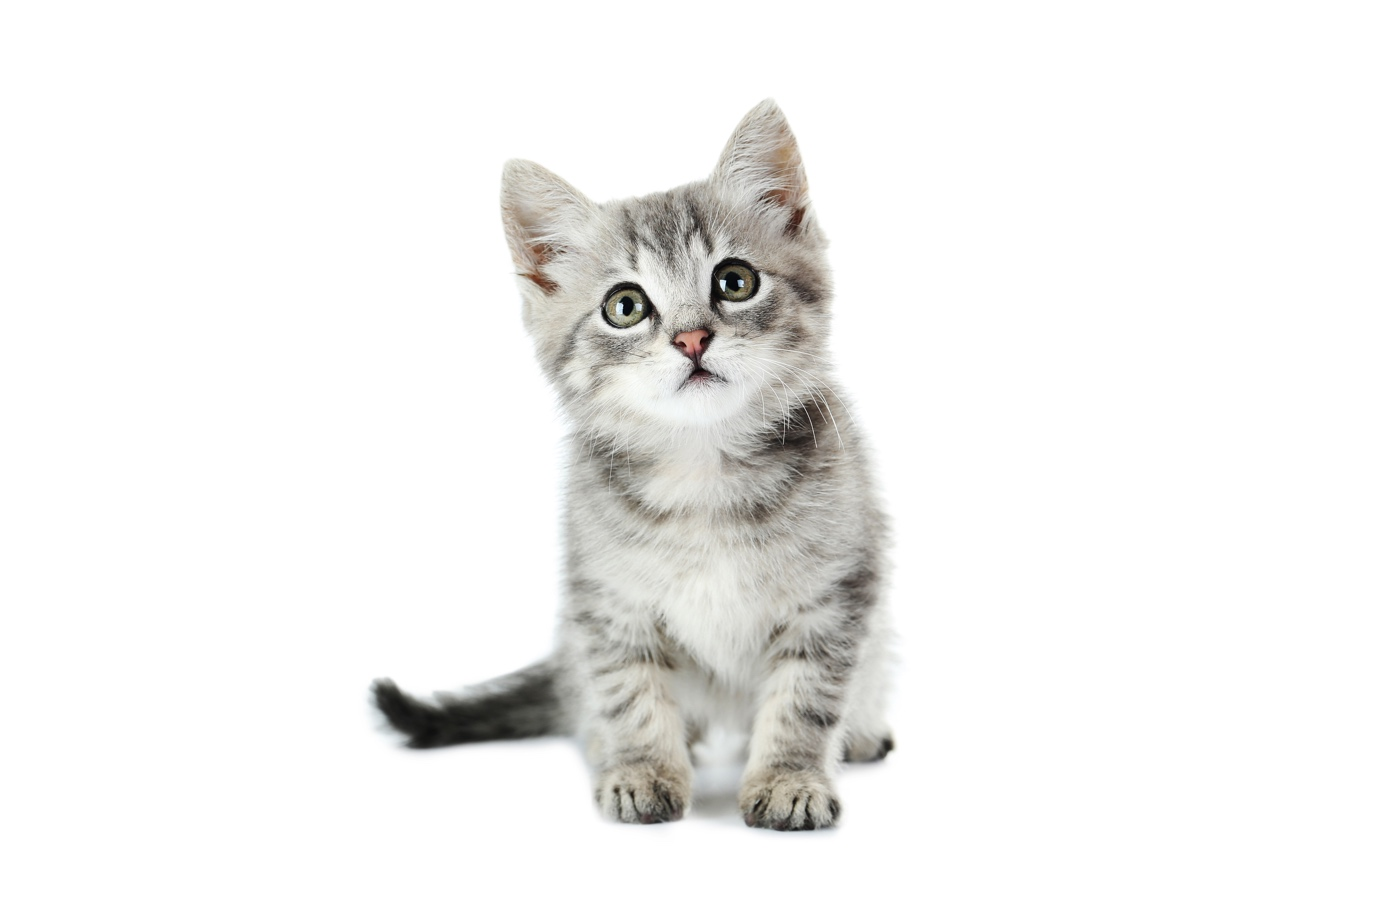
\includegraphics[width=0.3\textwidth,valign=c]{kitten.jpg}
    \end{align*}

    \begin{align*}
        x = \frac{-b \pm\sqrtsign{b^2 - 4ac}}{2a}.
    \end{align*}
    
    \begin{itemize}[left=-12pt, labelsep=23pt, label=\Huge\textbullet]
        \item We try to do this. what?
        \item we try to do that.
    \end{itemize}
}

\block{Section 2}{
    \lipsum[1]
}

\column{0.5}

\block{Section 3}{
    \textcolor{MainPurple}{\lipsum[1]}

}

\block{Conclusions}{
    \lipsum[1]
}

\end{columns}
\end{document}